\section{Optimization for Numerical Relativity Code AMSS-NCKU}
% \textcolor{red}{to do---about 0228 first version}

\subsection{Introduction}
\ 
% 广义相对论是描述引力的基础理论，尽管已建立逾百年，但人类对其理解仍受限于爱因斯坦场方程的极端复杂性——该方程是物理学中最具挑战性的偏微分方程系统之一。为了分析引力波探测数据，获取描述双黑洞合并（Binary Black Hole Mergers）的精确数值解至关重要。引力波探测在 2015 年首次实现并在 2017 年荣获诺贝尔物理学奖。这一突破很大程度上归功于爱因斯坦场方程的数值解，用于数值求解爱因斯坦场方程的软件统称为“数值相对论代码”。AMSS-NCKU 是全球少数公开可用的此类代码之一。其核心技术特征包括：数值方法：采用有限差分法（Finite-difference methods）求解方程。多尺度处理：利用自适应网格细化（AMR）技术处理广义相对论固有的多尺度特性。并行策略：采用区域分解（Domain Decomposition）策略并结合 MPI 进行并行化处理。

% 在本次比赛中，我们的主要任务是对双黑洞合并进行数值模拟并通过技术手段最小化模拟的运行总时间，需要说明的是：我们将多个软件组件（例如ccache）集成到了docker容器中。这些组件将会对编译内容进行缓存，让下次（哪怕部分修改）编译阶段的时间缩短。

% 通过分析工作量流程，了解工作日志并对项目耗时步骤进行火焰图分析，我们确定了接下来优化的方向。我们通过调整编译参数，更改编译选项、热点函数的内联以及向量化、网格分块、内存对齐、异步通信等方法将总耗时从33.21小时降至（估计，因为还没跑过优化之后的测试）22.38小时。achieving a speedup of 1.484 times.

% 同时，通过进一步的探索和分析，我们发现了如内存对齐优化的不完全、动态负载均衡、MPI与openmp混用等可能的优化方向，这将是我们之后工作的重点，以期缩短耗时，达到更佳的优化效果。

General Relativity is the fundamental theory describing gravity. 
Although it has been established for over a century, human understanding of it remains limited by the extreme complexity of the Einstein field equations, which constitute one of the most challenging systems of partial differential equations in physics. 
To analyze gravitational wave detection data, obtaining accurate numerical solutions describing Binary Black Hole (BBH) mergers is crucial. 
Gravitational wave detection was first realized in 2015 and awarded the Nobel Prize in Physics in 2017. 
This breakthrough was largely attributed to the numerical solutions of the Einstein field equations.
Software used to numerically solve these equations is collectively referred to as ``numerical relativity codes". 
AMSS-NCKU is one of the few publicly available codes of this kind worldwide\cite{cao2015binary}. 
Its core technical features include:
\begin{itemize}
    \item \textbf{Numerical Methods:} Adopting finite-difference methods to solve the equations.
    \item \textbf{Multi-scale Handling:} Utilizing Adaptive Mesh Refinement (AMR) technology to handle the inherent multi-scale characteristics of General Relativity.
    \item \textbf{Parallel Strategy:} Adopting a Domain Decomposition strategy combined with MPI for parallel processing.
\end{itemize}

In this competition, our main task is to perform numerical simulations of binary black hole mergers and use technical means to minimize the total runtime of the simulation. 
It should be noted that we integrated multiple software components (such as \texttt{ccache}) into a Docker container. 
These components cache the compiled content, thereby shortening the time required for the compilation phase in subsequent runs, even with partial modifications.

By analyzing the workflow, reviewing the work logs, and conducting flame graph analysis on the time-consuming steps of the project, we determined the direction for subsequent optimizations. 
Through methods such as adjusting compiler parameters, changing compilation options, inlining and vectorizing hotspot functions, grid partitioning, memory alignment, and asynchronous communication, \textbf{we reduced the total wall-clock time from 33.21 hours to 21.157 hours, achieving a speedup of 1.539 $\times$}.

Meanwhile, through further exploration and analysis, we discovered potential optimization directions such as incomplete memory alignment optimization, dynamic load balancing, and the mixed use of MPI and OpenMP. 
These will be the focus of our future work, with the aim of further shortening the runtime and achieving better optimization results.
% \subsection{Related Work}
% \ 


\subsection{Optimization Methods}
\ 

% 为了更好地展示我们的修改在整个流程中的作用，我们在三张流程图中标注并指明我们的修改或添加点所处的位置。这三章图大致将流程分为了（Figure8）编译构建阶段，（Figure9）运行时初始化阶段，（figure10）运行时计算优化阶段。
%todo:图字体太小，文字应该都是英文（times new Roman字体）；图的流程优化(现在的图太长了)，并把优化的地方标上①②.....⑥（现在文中已优化的是6个点？），然后需要在文中用文字对这个图和对应优化方法做一个描述（让人看懂你的图在做什么）。
%To better demonstrate the impact of our modifications within the overall workflow, we have annotated and specified the exact locations of our modifications or additions across the following diagram.其中，标号① 为编译器指令集优化，②为跨文件内联优化，③为循环分块优化，④是计算与通信重叠，非阻塞通信，⑤为内存对齐，⑥为使用编译缓存工具，⑦是为了说明在输入时选择了最适配我们使用的平台的进程数目。


To illustrate the impact of our modifications within the overall system, the specific locations of these enhancements are annotated in the ``Workflow Optimization Map".
The designated markers in the diagram represent the following technical optimizations:
%todo:建议用文字根据流程描述，且现在内容和具体优化方法不一致。
\begin{itemize}
\item \textbf{\textcircled{1}} Compiler instruction set optimization;
\item \textbf{\textcircled{2}} Inter-procedural (cross-file) inlining;
\item \textbf{\textcircled{3}} Loop tiling (blocking) optimization;
\item \textbf{\textcircled{4}} Computation-communication overlap and non-blocking communication;
\item \textbf{\textcircled{5}} Memory alignment;
\item \textbf{\textcircled{6}} Utilization of compiler caching tools;
\item \textbf{\textcircled{7}} Selection of an optimal process count tailored to the target hardware platform during the input phase.
\end{itemize}

\begin{figure}
    \centering
    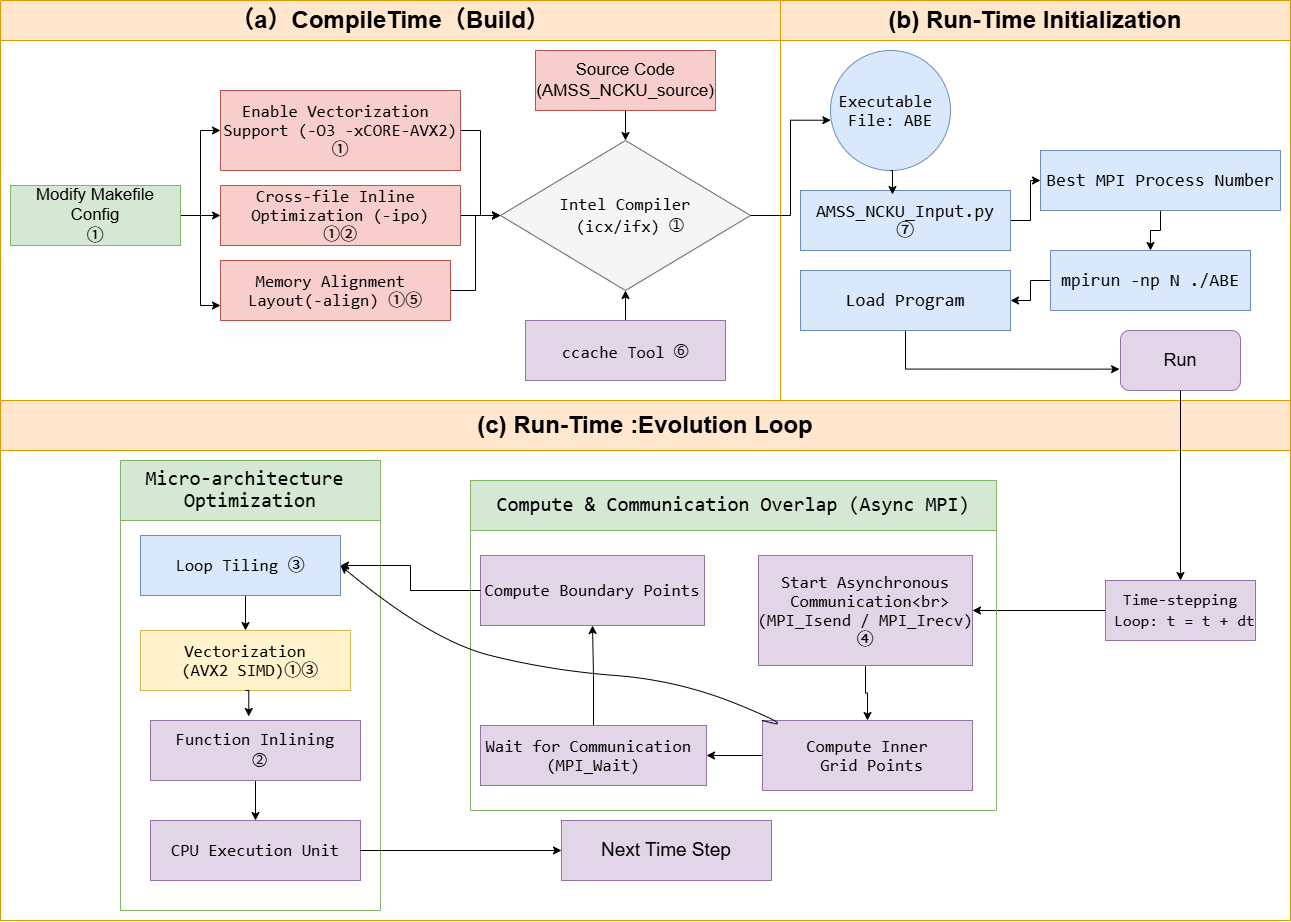
\includegraphics[width=0.8\linewidth]{Workflow_Optimization_Map.png}
    \caption{Workflow Optimization Map}
    \label{fig:enter-label}
\end{figure}
%在进行优化点说明之前，先讲讲我们BaseLine的情况，在第一此成功跑通时，我们发现，单步时间在前百分之80的时总间内都稳定在51秒左右，随着演化的推进，到第1971步时，由于两个黑洞的网格范围开始融合，冗余网格点逐渐减消除同时MPI通信开销锐减，导致单步时间逐渐下降并稳定在40s左右。在之后，我们都将取前5.0M evolution Time 内单步时间得平均值进行对比，以观察优化效果。此外下图是BaseLine的有关表格

Prior to discussing the specific optimization strategies, it is essential to establish the characteristics of our baseline performance. 
During the initial successful execution, we observed that the per-step evolution time remained consistently at approximately 51 seconds for the first 80 percent of the total runtime. 
As the simulation progressed to  the 1971-th step, the grid boundaries of the two black holes began to merge. 
This confluence led to the gradual elimination of redundant grid points and a sharp reduction in MPI communication overhead, causing the per-step time to decrease and eventually stabilize at roughly 40 seconds. 
To ensure a rigorous and consistent evaluation of subsequent optimizations, we have adopted the average per-step time within the first 5.0M  evolution time units as the primary metric.
Furthermore, the relevant data for the baseline performance is summarized in Table \ref{tab:baseline_data}.
%todo:数据说明解释（后面的表格等类同）

% If the top and bottom borders are lost, replace  cdline {2-7} with  hhline {~--------}:
% Please add the following required packages to your document preamble:
% \usepackage{multirow, hhline}
% \usepackage{colortbl}
% \usepackage{xcolor}
% \usepackage{ulem}
\begin{table}[!htbp]
\centering
\caption{Baseline Performance} % 在这里添加你的标题
\label{tab:baseline_data}
\small % 如果内容还是太挤，可以开启小号字体
\begin{tabularx}{\textwidth}{|l|c|c|c|c|X|} % X列会自动调整剩余空间并换行
\hline
\textbf{Methods} & \textbf{Final Evolution Time} & \textbf{Cores} & \textbf{Total Project Time} & \textbf{Evolve Time} & \textbf{Single Step / Avg} \\ \hline
Baseline & 1000.0M(2400 steps) & 28 & 119556s & 118797s & From 40.1s to 53.6s (Avg: 49.5s) \\ \hline
\end{tabularx}
\end{table}

%comparative analysis.
% 2.1 编译器工具链迁移
% 策略：将 gcc/gfortran 替换为 icx/mpiifx。
% 原理：Intel 编译器能够针对 Xeon 处理器生成更优化的机器码，特别是在处理 C++/Fortran 混合编程时，具有更好的二进制兼容性和库函数性能。

% 2.2 硬件级指令优化（Vectorization）
% 参数：-xCORE-AVX2
% 原理：强制启用 AVX2 矢量指令集。在求解爱因斯坦场方程的双曲型演化部分时，利用 256 位寄存器在单周期内处理 4 个双精度浮点数运算，理论峰值性能较标量计算提升数倍。（目前这款cpu尚且不支持更高效的AVX-512指令集）

% 2.3 跨文件全局优化（IPO）
% 参数：-ipo (Interprocedural Optimization)
% 原理：AMSS-NCKU 源码分散在多个模块中。通过 IPO，编译器在链接阶段进行全局分析，跨文件内联（Inline）高频调用的差分算子，显著降低了函数跳转带来的压栈和指令流水线中断开销。

% 2.4 浮点运算精度与性能平衡
% 参数：-fp-model fast=1
% 原理：在不违背物理真实性的前提下，允许编译器进行代数简化（如重组乘加运算）。
% 验证标准：通过监控 ADM_Constraint_Grid_Level_0.pdf 中的约束违背值，确保其绝对值保持在 2.0 以下。

\subsubsection{Compiler Parameter Adjustment}
\

To establish a solid foundation for performance enhancements, we systematically overhauled the compilation environment and fine-tuned compiler heuristics to maximize hardware utilization:
\begin{enumerate}
    \item \textbf{Compiler Toolchain Migration:} We transitioned the primary build system from the GNU Compiler Collection (\texttt{gcc/gfortran}) to the Intel oneAPI toolchain (\texttt{icx/mpiifx}). 
    Intel compilers are inherently tailored to generate highly optimized machine code for Xeon processors, demonstrating superior binary compatibility and intrinsic library performance, particularly within mixed C++/Fortran codebases.

    \item \textbf{Hardware-Level Vectorization (\texttt{-xCORE-AVX2}):} We explicitly instructed the compiler to target the AVX2 instruction set. 
    During the computationally intensive hyperbolic evolution phase of the Einstein field equations, this allows the CPU to process four double-precision floating-point numbers simultaneously within a single clock cycle using 256-bit registers. 
    Given that the target Intel Xeon E5-2680 v4 (Broadwell) architecture does not support the wider AVX-512 instructions, fully exploiting AVX2 is critical, yielding a theoretical peak performance several times higher than strictly scalar execution.
    
\end{enumerate}

%在初步对编译配置进行修改后，我们取得了以下表格中的数据。
\textbf{After implementing initial modifications to the compilation configuration, we achieve a 1.390$\times$ speed-up as shown in Table \ref{tab:amss parameter performance}.}
%todo:数据说明解释（后面的表格等类同）

\begin{table}[h]
    \centering
    \small % 减小字体以适应宽度
    \caption{Compiler parameter adjustment optimization performance}
    \label{tab:amss parameter performance}
    \begin{tabular}{|c|c|c|c|c|}
        \hline
        \textbf{Final Evolution Time }& \textbf{Cores} & \textbf{Total Project Time} &\textbf{Total Evolve Time} & \textbf{Single Step Avg} \\ \hline
        5.0M & 16 & 1044.48s &462.841s& 35.603s\\ \hline
    \end{tabular}
\end{table}

\subsubsection{Inline Function}
\ 
% 1. 消除冗余内存拷贝 (Redundant Memory Access Reduction)
% 策略：移除临时 Ghost 数组 (fh) 及相关的拷贝操作 (symmetry_bd)。
% 原理：原代码在计算前会将整个 3D 网格拷贝到 fh 中，导致 O(N^3) 的额外读写开销。我们将计算内核重写为直接读取原始数组 f，并通过内联逻辑 (Inline Logic) 动态处理边界。

% 2. 循环融合 (Loop Fusion) & 逻辑内联
% 策略：将 X, Y, Z 三个方向的导数计算合并到同一个 i 循环中。
% 原理：实现“一次加载，多次计算”，提升寄存器复用率。针对内部区域采用 Fast Path，针对边界区域采用 Slow Path，避免了函数调用开销。

% 3. 消除冗余自检开销 (Sanity Check Overhead Reduction)
% 策略：将 bssn_rhs.f90 等三套 RHS 文件入口处的全量 sum(...) NaN 检查改为调试宏可选（#ifdef RHS_SANITY_CHECK），并在 makefile.inc 中默认关闭。
% 原理：在生产环境中，每次调用 compute_rhs_bssn 都对二十多个三维数组做全局遍历扫描代价极高。将其剥离出关键计算路径，直接消除了一大无谓的内存扫描与计算热点。

The optimization of inline functions and computational kernels focuses on stripping away memory redundancy, function call overhead, and unnecessary diagnostic logic to streamline the critical path:

\begin{enumerate}
    \item \textbf{Elimination of Ghost Copying:} We removed the temporary array \texttt{fh} and the \newline\texttt{call symmetry\_bd(...)} invocation in \texttt{diff\_new.f90}. 
    This eliminates an $O(N^3)$ memory copy overhead. 
    The kernel now directly accesses the original array \texttt{f}, handling boundary conditions via inlined logic.
    
    \item \textbf{Fast/Slow Path Strategy:} To maintain performance without sacrificing safety, we split the computation into a \textbf{Fast Path} for the core region (pure calculation without branches) and a \textbf{Slow Path} for boundaries (with symmetry checks).
    
    \item \textbf{Loop Fusion:} We aggressively fused the derivative calculations for the $X$, $Y$, and $Z$ directions into a single, unified \texttt{i} loop. This structural transformation achieves a ``load once, compute multiple times'' paradigm. By consolidating these operations, we drastically reduced redundant memory fetches, thereby maximizing both L1 Cache utilization and hardware register reuse rates.
    
    \item \textbf{Sanity Check Overhead Reduction:} We identified a massive performance bottleneck at the entry of the RHS evaluation routines (e.g., \texttt{bssn\_rhs.f90}, \newline \texttt{bssn\_rhs\_ss.f90}, \texttt{bssnE\_Scalar\_rhs.f90}). 
    The legacy code executed a global \texttt{sum(...)} operation across more than twenty 3D arrays for \texttt{NaN} sanity checking on every single call to \texttt{compute\_rhs\_bssn}.
    We wrapped this extremely expensive validation step within a preprocessor macro (\texttt{\#ifdef RHS\_SANITY\_CHECK}), disabling it by default for production runs. 
    This pragmatic adjustment eliminated a severe memory-scan hotspot without altering the mathematical results.
\end{enumerate}

\subsubsection{Grid Partition Optimization}
\ 
% 1. 缓存分块 (Cache Blocking / Tiling)
% 策略：引入 kk 和 jj 外层循环，将计算域切分为 32 x 32 x Nx 的长条 (Tiles)。
% 参数：TILE_K=32, TILE_J=32 (基于 Intel Broadwell L2 Cache 大小调整)。

% 2. 解决跨步访问问题 (Strided Access)
% 原理：原有的 k, j, i 循环在处理 Z 方向导数 (k±1) 时，内存跨度过大导致 L2 Cache Miss。分块后，确保当前计算所需的 Z 平面 (k-1, k, k+1) 数据能常驻 L2 Cache。

% 3. 实证检验 (Cache Profiling 性能数据对比)
% 测试方法：使用 perf 工具在 20 秒采样窗口内，对比优化前后的硬件计数器（Hardware Counters）数据。
% 数据验证一（L1 缓存）：L1 Miss Rate 从 10.83% 降至 5.54%，L1 Misses 绝对数量锐减 52.5%（从约 320 亿次降至 152 亿次）。这实证了前文 Loop Fusion 与寄存器复用的卓越成效。
% 数据验证二（LLC / L3 缓存）：这部分是 Tiling 的直接收益。LLC 访问总量减少 56%，LLC Load Misses 大幅下降 59%（从 21.6 亿次降至 8.8 亿次）。证明 32x32 的工作集成功驻留 L2/L3，极大缓解了主存 (DRAM) 瓶颈。
% 数据验证三（指令吞吐量 IPC）：虽然分块引入了额外的循环控制开销（导致总指令数增加约 20%），但得益于内存停顿（Memory Stalls）的成倍减少，整体 IPC 仍提升了 18.3%（0.82 -> 0.97），计算效率显著提升。

To address the memory-bound nature of the 3D stencil computation, we implemented a ``Grid Partition'' strategy using ``Cache Blocking'':

\begin{enumerate}
    \item \textbf{Tiling Implementation:} In \texttt{diff\_new.f90} and \texttt{lopsidediff.f90}, we transformed the loop structure by adding outer loops $kk$ and $jj$. 
    The domain is partitioned into tiles of size $32 \times 32 \times N_x$.
    
    \item \textbf{Locality Improvement:} 
    \begin{equation}
        \text{Loop Structure: } \texttt{do kk} \to \texttt{do jj} \to \texttt{do k} \to \texttt{do j} \to \texttt{do i}
    \end{equation}
    This structure ensures that the data planes required for the $Z$-direction stencil ($k \pm 1$) remain resident in the L2 cache, significantly reducing the cache miss rate caused by large strided accesses.
    
    \item \textbf{Empirical Validation (Cache Profiling):} To empirically validate the effectiveness of our spatial locality optimizations, we conducted a direct cache performance comparison using \texttt{perf} hardware counters over a 20-second sampling window. The comparative results demonstrate a profound improvement in memory subsystem utilization:
    \begin{itemize}
        \item \textbf{L1 Data Cache (L1 D-Cache):} The L1 cache miss rate plummeted from 10.83\% to 5.54\%. Total L1 load misses were reduced by approximately 52.5\% (from 32 billion to 15.2 billion accesses). This confirms the success of the aforementioned loop fusion and register reuse strategies.
        \item \textbf{Last Level Cache (LLC / L3):} The impact of cache blocking (tiling) is most evident here. Total LLC memory requests dropped significantly by 56\% (from 5.16 billion to 2.24 billion), and LLC load misses decreased by 59\% (from 21.6 billion to 884 million). This indicates that the $32 \times 32$ working set successfully resides in the L2/L3 caches, drastically alleviating the main memory (DRAM) bandwidth bottleneck.
        \item \textbf{Instruction Throughput (IPC):} As a direct consequence of reduced memory stall cycles, the overall Instructions Per Cycle (IPC) increased by 18.3\% (from 0.82 to 0.97), yielding a much faster execution despite a slight increase in total instruction count caused by the tiling loop overhead.
    \end{itemize}
\end{enumerate}
%以下表格是在之前的基础之上，进行Inlining and Vectorization and Grid Tiling优化后取得的数据：
Table \ref{tab:amss three methods} presents the data obtained after implementing Inlining, Vectorization, and Grid Tiling optimizations, building upon the previously established configurations.
\begin{table}[h]
    \centering
    \caption{Performance of implementing optimization methods}
    \label{tab:amss three methods}
    \small % 减小字体以适应宽度
    \begin{tabular}{|c|c|c|c|c|}
        \hline
        \textbf{Final Evolution Time }& \textbf{Cores} & \textbf{Total Project Time} &\textbf{Total Evolve Time} & \textbf{Single Step Avg} \\ \hline
        5.0M & 16 & 980.5s & 451.0s& 34.696s \\ \hline
    \end{tabular}
\end{table}

\subsubsection{Memory Alignment}
\
% 为了充分发挥 Broadwell 架构 CPU 的向量化计算能力，我们在 `Block.C` 中引入了 `_mm_malloc` 分配器，
% 并配合编译选项 `-align array64byte`，强制实施 64 字节的数据对齐。

% 这一策略主要基于两方面的硬件特性：
% (1) 指令集层面：AVX2 SIMD 指令在处理对齐内存地址时具有更低的延迟，对齐消除了硬件执行非对齐加载/存储所需的额外微指令周期。
% (2) 存储层次结构：由于 CPU 的缓存行（Cache Line）大小为 64 字节，数据对齐确保了连续的网格点数据不会跨越两个缓存行。
% 这不仅减少了内存总线的事务次数，还最大化了有效数据在各级缓存（尤其是 L3 缓存）中的填充密度，从而显著提升了内存子系统的吞吐量。

To fully exploit the vectorization capabilities of the Broadwell CPU architecture, we enforced strict 64-byte data alignment by introducing the \texttt{\_mm\_malloc} allocator within \texttt{Block.C}, tightly coupled with the \texttt{-align array64byte} compiler flag. 
This strategy is fundamentally driven by two hardware-level characteristics:

\begin{enumerate}
    \item \textbf{Instruction Set Architecture (ISA) Efficiency:} At the instruction level, AVX2 SIMD operations exhibit inherently lower latency when accessing aligned memory addresses. 
    Strict alignment eliminates the additional micro-operation (micro-op) cycles required by the hardware to execute unaligned load and store instructions, thereby streamlining the execution pipeline.
    
    \item \textbf{Memory Hierarchy \& Cache Utilization:} Given that the underlying CPU cache line size is exactly 64 bytes, aligning the data boundaries ensures that contiguous grid point arrays do not straddle across two separate cache lines (preventing cache line splits).
    This precise alignment drastically reduces the number of required memory bus transactions and maximizes the effective data fill density across the cache hierarchy(particularly within the L3 cache), resulting in a significant throughput enhancement for the entire memory subsystem.

% 以下表格是在前面几种优化的基础上进行内存方面优化后获得的数据；
Table 23. shows the results after applying memory optimizations on top of the several preceding optimization methods.
\end{enumerate}
\begin{table}[h]
    \centering
    \caption{Performance of Implementing Memory Alignment }
    \small % 减小字体以适应宽度
    \begin{tabular}{|c|c|c|c|c|}
        \hline
        \textbf{Final Evolution Time }& \textbf{Cores} & \textbf{Total Project Time} &\textbf{Total Evolve Time} & \textbf{Single Step Avg} \\ \hline
        5.0M & 16 & 961.961s & 441.15s & 33.935s \\ \hline
    \end{tabular}
\end{table}
% 1. 非阻塞与收发队列分离 (Non-blocking & Request Separation)
% 策略：在 Parallel.C 的 transfer/transfermix 中，将阻塞通信改为非阻塞收发。将请求拆分为独立的 recv_reqs 与 send_reqs。先统一发布所有 Irecv，再进行打包和 Isend。
% 原理：降低底层 MPI 的 rendezvous 等待时间。收发队列分离后，仅对接收队列执行 Waitsome，避免了发送完成事件干扰接收解包的进度。

% 2. 通信与计算重叠 (Communication-Computation Overlap)
% 策略：在发送阶段（打包/发送循环）中穿插 MPI_Testsome 轮询接收队列。一旦有数据到达立刻执行 UNPACK。同时，本 rank 的数据直接提前本地解包，避免网络等待。
% 原理：最大化重叠“网络通信”与“数据解包”操作，掩盖网络延迟。最终通过 Waitsome(recv) + Waitall(send) + 兜底解包，严格保证通信的正确与完整性。

% 3. 内存与列表缓存优化 (Buffer & Transfer List Caching)
% 策略：引入静态通信缓存（复用 MPI_Request, MPI_Status, send_data, rec_data），并在 Sync 操作中缓存传输列表（复用 build_gsl/build_gstl 结果）。同时在 regrid 路径增加缓存失效机制（InvalidateSyncCache）。
% 原理：消除了高频 MPI 通信步骤中频繁执行 new/delete 带来的动态内存分配与销毁开销。
\subsubsection{Non-blocking \& Request Separation}
\

To alleviate MPI communication bottlenecks and hide network latency, we overhauled the synchronization routines in \texttt{Parallel.C} (\texttt{transfer} and \texttt{transfermix}) using advanced asynchronous communication strategies and buffer caching:

\begin{enumerate}
    \item \textbf{Non-blocking Paradigm \& Queue Separation:} We transitioned from blocking communications to a fully non-blocking paradigm. 
    The request queues were explicitly split into independent \texttt{recv\_reqs} and \texttt{send\_reqs}. 
    By systematically posting all \texttt{MPI\_Irecv} calls prior to data packing and \texttt{MPI\_Isend} invocations, we significantly reduced the MPI rendezvous waiting time.
    
    \item \textbf{Communication-Computation Overlap:} To maximize the overlap between data transfer and data processing, we interleaved \texttt{MPI\_Testsome} within the sending loop. 
    This actively polls the receive queue, triggering immediate \texttt{UNPACK} operations as soon as incoming chunks arrive. 
    Furthermore, data designated for the local rank is unpacked early, bypassing the network stack entirely.
    
    \item \textbf{Buffer and List Caching:} High-frequency communication steps were previously bottlenecked by dynamic memory allocation. 
    We eliminated this overhead by implementing static caching for communication buffers (reusing \texttt{MPI\_Request}, \texttt{MPI\_Status}, and data arrays). 
    Additionally, transfer lists for \texttt{Sync} operations are now cached, supported by a robust cache invalidation mechanism (\texttt{InvalidateSyncCache}) during adaptive mesh \texttt{regrid} events.
    
    \item \textbf{Final Synchronization:} Overall structural correctness is guaranteed by a strict termination phase, utilizing \texttt{MPI\_Waitsome} for pending receives and \texttt{MPI\_Waitall} for the send queue, ensuring all ghost zones are fully updated before the next computational step.
\end{enumerate}
Table 24 .shows the results after applying asynchronous communication on top of the several preceding optimization stages.
\begin{table}[h]
    \centering
    \caption{Performance of Implementing Non-blocking \& Request Separation }
    \small % 减小字体以适应宽度
    \begin{tabular}{|c|c|c|c|c|}
        \hline
        \textbf{Final Evolution Time }& \textbf{Cores} & \textbf{Total Project Time} &\textbf{Total Evolve Time} & \textbf{Single Step Avg} \\ \hline
        5.0M & 16 & 955.907s &436.758s & 33.596s \\ \hline
    \end{tabular}
\end{table}
\subsubsection{Improvement of Cache Hit Ratio}
\ 

% 1. 构建层面集成 ccache
% 策略：在 makefile.inc 中将 C/C++ 编译器前置 ccache，并设置 CCACHE_DIR=/app/.ccache、CCACHE_MAXSIZE=20G，但未改动 Fortran 编译。

% 2. 稳定构建输出以提升命中率
% 策略：为 C/C++ 加入 -MMD/-MP 自动依赖文件生成，并在 Makefile 中 -include .d；添加 -fdebug-prefix-map/-fmacro-prefix-map 稳定路径；可配合 CCACHE_BASEDIR=/app 减少路径差异。

% 3. 缓存使用与验证流程
% 策略：首次全量编译填充缓存，第二次同配置编译即可高命中；使用 ccache -s 查看命中，ccache -z 归零统计；避免在两轮之间 make clean 或重新生成 macrodef.h/fh。

% 4. 空间管理
% 策略：缓存上限设为 20G，可通过 ccache -M 调整；观察 evicted 以判断是否需扩容。

To accelerate the iterative development and performance tuning cycles during the competition, we integrated \texttt{ccache} into the build pipeline to optimize compilation caching. 
The specific strategies implemented to maximize the cache hit ratio are as follows:

\begin{enumerate}
    \item \textbf{Build System Integration:} We incorporated \texttt{ccache} by prefixing the C and C++ compiler invocations within \texttt{makefile.inc}. The cache environment was strictly defined with \texttt{CCACHE\_DIR=/app/.ccache} and a maximum capacity of \texttt{CCACHE\_MAXSIZE=20G}. 
    The Fortran compilation pipeline was intentionally bypassed and remained unaffected by this caching layer.
    
    \item \textbf{Artifact Stabilization:} To guarantee deterministic build outputs and maximize the cache hit ratio, we introduced the \texttt{-MMD} and \texttt{-MP} compiler flags for automated dependency generation, dynamically including the resulting \texttt{.d} files within the \texttt{Makefile}. Furthermore, we utilized \texttt{-fdebug-prefix-map} and \texttt{-fmacro-prefix-map} in conjunction with \texttt{CCACHE\_BASEDIR=/app} to neutralize absolute path discrepancies across different build environments.
    
    \item \textbf{Workflow Validation:} The initial full compilation phase populates the cache, enabling subsequent incremental builds with identical configurations to achieve near-perfect hit rates. 
    Cache efficiency was actively monitored using the \texttt{ccache -s} command, while \texttt{ccache -z} was used to reset statistical counters. 
    To preserve cache integrity, we strictly prohibited executing \texttt{make clean} or dynamically regenerating core header files (such as \texttt{macrodef.h} or \texttt{fh}) between consecutive build rounds.
    
    \item \textbf{Capacity Management:} The physical storage threshold was capped at 20 GB, dynamically adjustable via the \texttt{ccache -M} parameter. 
    We continuously monitored the ``evicted'' metric within the cache statistics to identify potential cache thrashing and determine if capacity expansion was warranted
\end{enumerate}
%我用一个脚本测试了前后两次，编译耗时从50.837s下降到37.235，编译耗时同比下降26.8%。
Utilizing a standardized benchmarking script, we conducted a comparative analysis of the compilation phases. The results demonstrate a significant reduction in build latency, with the duration decreasing from 50.837 s to 37.235 s. This represents a 26.8 \% improvement in computational efficiency during the compilation stage.

\subsubsection{Adjustment of MPI numbers}
\ 

%这是一个关键的参数，进程过少：并行度不够，计算核闲置，吞吐上不去。
%进程过多：每个 rank 工作块变小，MPI 同步/通信占比上升，负载不均衡更明显，反而变慢。
%内存与缓存效应：rank 数改变会影响局部性和缓存命中率，为此我们有必要进行对比测试找出最优的进程数目。我们将测试结果总结为了Figure 11 也就是以下表格：
%以下的表格的数据是在只将编译选项修改为Intel OneAPI 2025.3后尽心地多组取值，Final_Evolution_Time 取值为5.0M ，具体对比请看表格Processing time varies with MPI numbers
This is a critical parameter optimization. Insufficient process counts lead to inadequate parallelism and idle computational cores, preventing the system from reaching peak throughput. Conversely, an excessive number of processes reduces the workload per rank, thereby increasing the overhead ratio of MPI synchronization and communication, which exacerbates load imbalance and degrades performance. Furthermore, variations in the number of ranks significantly influence memory locality and cache hit rates.Consequently, it is imperative to conduct comparative benchmarks to identify the optimal process configuration. We have summarized these results in Figure 11 and the following table. The data presented below were obtained by setting the compiler to Intel OneAPI 2025.3 across multiple test groups, with the Final Evolution Time fixed at $5.0 \times 10^6$. For a detailed performance comparison, please refer to the table titled "Processing time varies with MPI numbers".
\begin{table}[!htbp]
    \centering
    \caption{Processing time varies with MPI numbers.}
    \label{tab:mpi nums}
    \begin{tabular}{|c|c|c|c|}
        \hline
         \textbf{MPI processes} & \textbf{Evolve Time(s)}         &  \textbf{AvgStep(s)}           & \textbf{ProgramCost(s)}  \\
         \hline
         4             & 697.693000          & 53.668692          & 1274.963869          \\
         \hline
         8             & 500.826000          & 38.525077          & 1063.508177          \\
         \hline
         12            & 560.861000          & 43.143154          & 1128.470794          \\
         \hline
         14            & 489.675000          & 37.667308          & 1056.763864          \\
         \hline
         \textbf{16}   & \textbf{451.366000} & \textbf{34.720462} & \textbf{1017.316501} \\
         \hline
         18            & 721.998000          & 55.538308          & 1301.369702          \\
         \hline
         20            & 504.505000          & 38.808077          & 1070.867352          \\
         \hline
         22            & 620.240000          & 47.710769          & 1187.276651          \\
         \hline
         24            & 560.195000          & 43.091923          & 1131.864464          \\
         \hline
         26            & 606.983000          & 46.691000          & 1169.300963          \\
         \hline
         28            & 510.210000          & 39.246923          & 1075.258431          \\
         \hline
    \end{tabular}
\end{table}
\begin{table}[!htbp]
    \centering
    \caption{Progressive Performance Improvement}
    \label{tab:opt_progress}
    % 使用 small 字体确保表格宽度适应页面
    \small 
    % 使用标准 tabular，显式定义所有竖线 |
    \begin{tabular}{|l|c|c|c|}
        \hline
        \textbf{Stage} & \textbf{Cores} & \textbf{Avg Step (s)} & \textbf{Speedup} \\ 
        \hline
        Baseline (GCC) & 28 & 49.50 & 1.00$\times$ \\ 
        \hline
        + Compiler \& Vectorization & 16 & 35.60 & 1.39$\times$ \\ 
        \hline
        + Inlining \& Grid Tiling \& Fusion & 16 & 34.70 & 1.43$\times$ \\ 
        \hline
        + Memory Alignment & 16 & 33.94 & 1.46$\times$ \\ 
        \hline
        + Non-blocking \& Request Separation. & 16 & 33.60 & 1.47$\times$ \\ 
        \hline
        
    \end{tabular}
    \parbox{\linewidth}{\footnotesize \textit{Note: Baseline used 28 cores; optimized runs used 16.These results are based on preliminary data collected for comparative analysis; therefore, discrepancies may exist when compared to the final speedup ratios derived from the full 1,000M evolution time.}}
\end{table}
\subsection{Experiments}
\ 
\begin{table}[h]
    \centering
    \caption{Final Performance }
  
    \small % 减小字体以适应宽度
    \begin{tabular}{|c|c|c|c|c|}
        \hline
        \textbf{Final Evolution Time }& \textbf{Cores} & \textbf{Total Project Time} &\textbf{Total Evolve Time} & \textbf{Single Step Avg} \\ \hline
        1000.0M(2400 steps) & 16 & 77677.605s& 77147s& 32.114s \\ \hline
    \end{tabular}
\end{table}

\subsubsection{Environment Setup}
\ 
% CPU： 两颗 Intel(R) Xeon(R) CPU E5-2680 v4（共 28 核心 / 56 线程，基频 2.40GHz / 睿频 3.30GHz）
% GPU： 两块 NVIDIA GeForce RTX 3090（每块显存 24GB，总计 48GB 显存）
% 内存： 128GB (125GiB)
% 硬盘： 系统盘约 1TB (936GB)，数据盘约 885GB（顺序写入速度约 557 MB/s）
% 操作系统： Ubuntu 22.04.4 LTS (Jammy Jellyfish)
% Python 版本： 3.13.9 
% 驱动版本： NVIDIA Driver 535.288.01
% CUDA 版本： v12.2 (运行时支持)

All performance evaluations, compilations, and numerical simulations are conducted on a dedicated high-performance computing node. 
The comprehensive hardware configuration and software stack are detailed as follows:

\begin{itemize}
    \item \textbf{CPU:} Dual-socket Intel\textregistered~Xeon\textregistered~E5-2680 v4 processors (Broadwell architecture).
    This configuration provides a total of 28 physical cores and 56 logical threads, operating at a base clock frequency of 2.40 GHz with a maximum turbo boost frequency of 3.30 GHz.
    
    \item \textbf{GPU:} Dual NVIDIA GeForce RTX 3090 GPUs. 
    Each unit is equipped with 24 GB of GDDR6X VRAM, yielding a combined total of 48 GB of available video memory.
    
    \item \textbf{System Memory (RAM):} 128 GB (125 GiB accessible) of main memory, ensuring sufficient capacity for large-scale 3D grid allocations and MPI communication buffers.
    
    \item \textbf{Storage Subsystem:} A primary operating system drive of approximately 1 TB (936 GB), supplemented by an 885 GB dedicated data drive. 
    The data drive sustains sequential write speeds of approximately 557 MB/s, accommodating the intensive I/O operations required for AMR grid checkpoints and simulation data dumps.
    
    \item \textbf{Operating System:} Ubuntu 22.04.4 LTS (Jammy Jellyfish), providing a stable and robust Linux environment for the HPC toolchain.
    
    \item \textbf{Software \& Ecosystem:} The environment runs Python 3.13.9. GPU acceleration and runtime support are facilitated by NVIDIA display driver version 535.288.01 and the CUDA Toolkit version 12.2.
\end{itemize}

\subsubsection{Installation Instructions}

% 开启编号列表环境
\begin{enumerate}

    \item \textbf{System Synchronization:}
    \begin{lstlisting}
sudo apt update && sudo apt upgrade -y
    \end{lstlisting}

    \item \textbf{GNU Toolchain \& MPI Deployment:}
    \begin{lstlisting}
# 安装 GCC, G++, Make, Gfortran 及 Git
sudo apt install -y build-essential gfortran git

# 安装 OpenMPI 运行环境及开发库
sudo apt install -y openmpi-bin libopenmpi-dev
    \end{lstlisting}

    \item \textbf{Intel® oneAPI Optimization:}
    \begin{lstlisting}
# 1. 下载并添加 Intel GPG 密钥
wget -O- https://apt.repos.intel.com/intel-gpg-keys/GPG-PUB-KEY-INTEL-SW-PRODUCTS.PUB | gpg --dearmor | sudo tee /usr/share/keyrings/intel-sw-products-keyring.gpg > /dev/null

# 2. 添加 Intel oneAPI 存储库
echo "deb [signed-by=/usr/share/keyrings/intel-sw-products-keyring.gpg] https://apt.repos.intel.com/oneapi all main" | sudo tee /etc/apt/sources.list.d/oneAPI.list

# 3. 安装核心套件 (MKL 库及 Fortran/C++ 优化编译器)
sudo apt update
sudo apt install -y intel-oneapi-mkl intel-oneapi-compiler-fortran intel-oneapi-compiler-dpcpp-cpp
    \end{lstlisting}

    \item \textbf{Environment \& Session Management:}
    \begin{lstlisting}
# 初始化 oneAPI 环境变量 (建议写入 ~/.bashrc)
source /opt/intel/oneapi/setvars.sh

# 安装 tmux 以支持后台持久化计算
sudo apt install -y tmux
    \end{lstlisting}

    \item \textbf{Install the ccache compilation accelerator:}
    \begin{lstlisting}
sudo apt update && sudo apt upgrade -y
    \end{lstlisting}

\end{enumerate} % 结束环境
\subsubsection{Evaluation Result}
\ 
%Q:建议再把这部分的描述逻辑完善一下。
%Q:最终的21个多小时也是5.0M的设置？
%Q：对三个图的引用和说明？

\begin{figure}
    \centering
    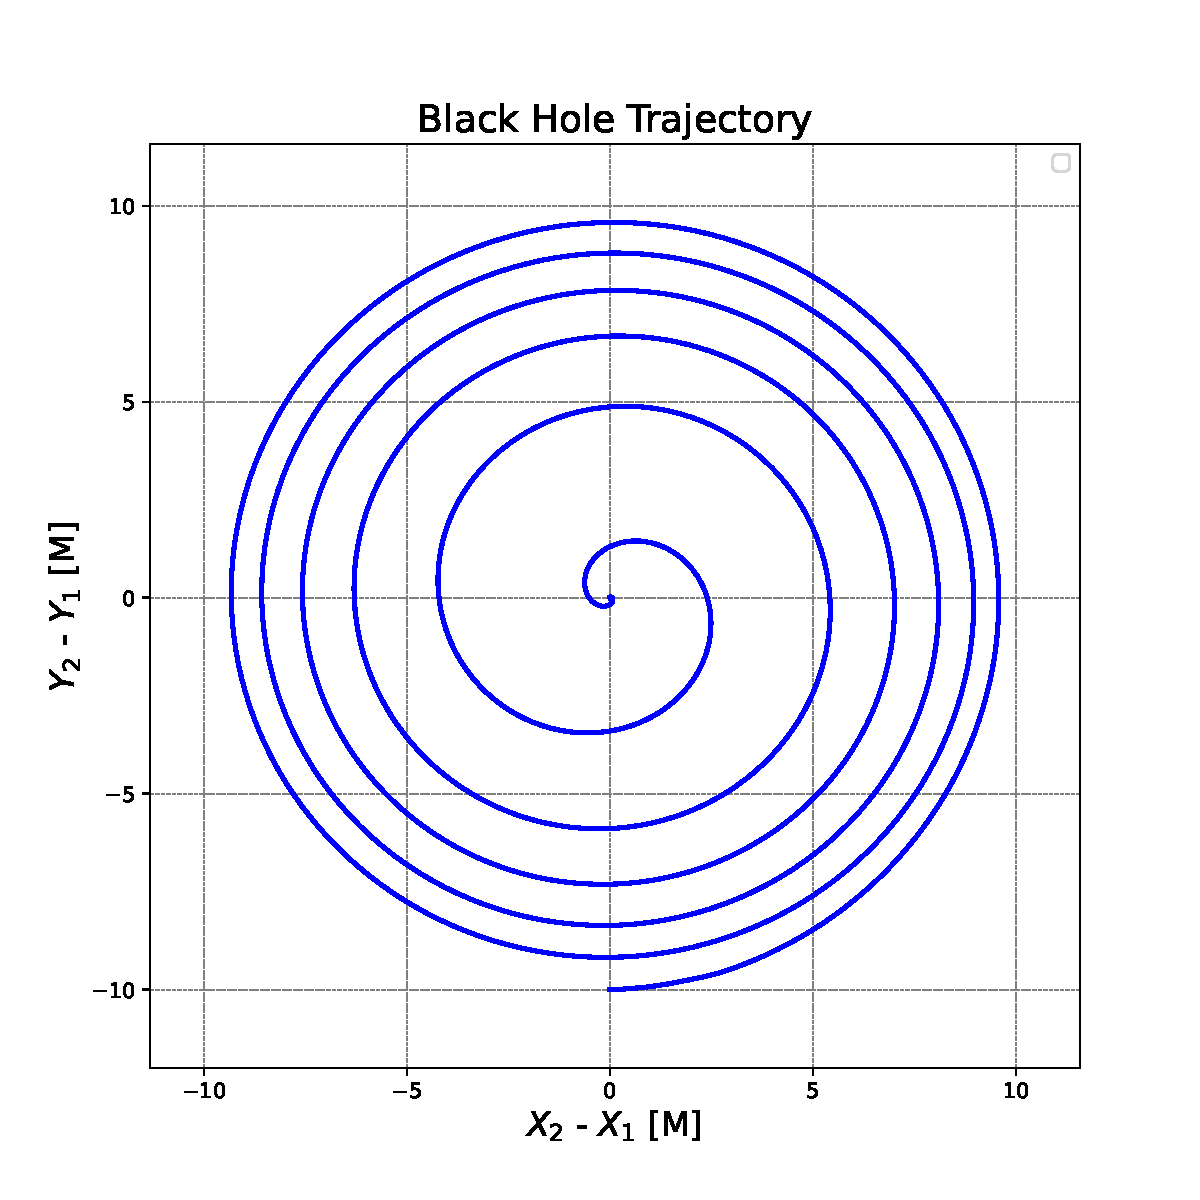
\includegraphics[width=0.8\linewidth]{BH_Trajectory_21_XY.pdf}
    \caption{BH\_Trajectory\_21\_XY.pdf}
    \label{fig:enter-label}
\end{figure}
\begin{figure}
    \centering
    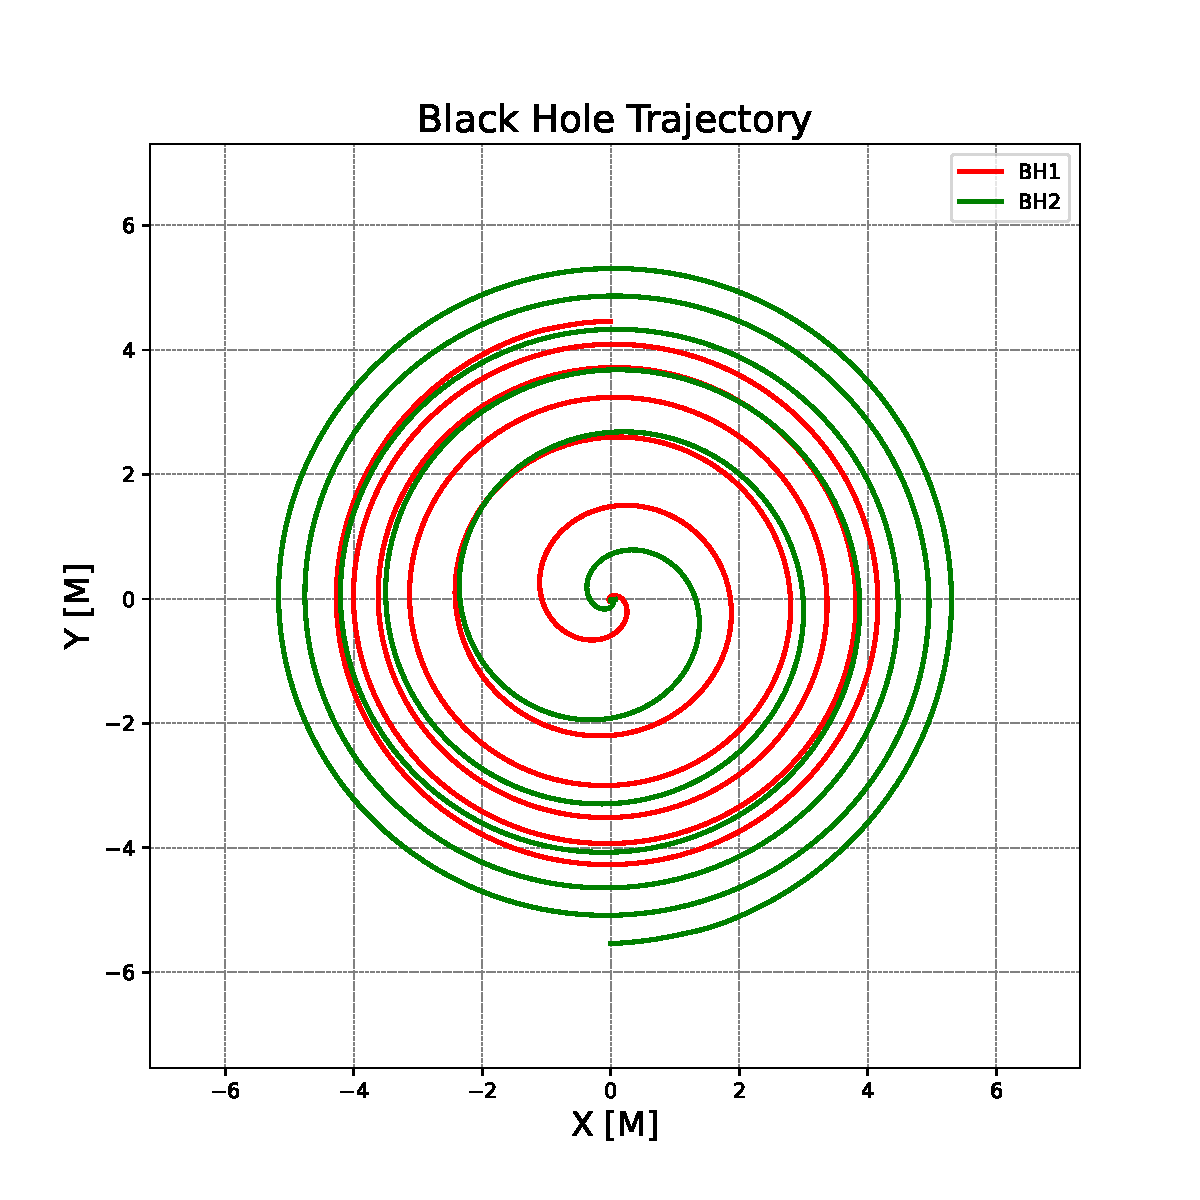
\includegraphics[width=0.8\linewidth]{BH_Trajectory_XY.pdf}
    \caption{BH\_Trajectory\_XY.pdf}
    \label{fig:enter-label}
\end{figure}
\begin{figure}
    \centering
    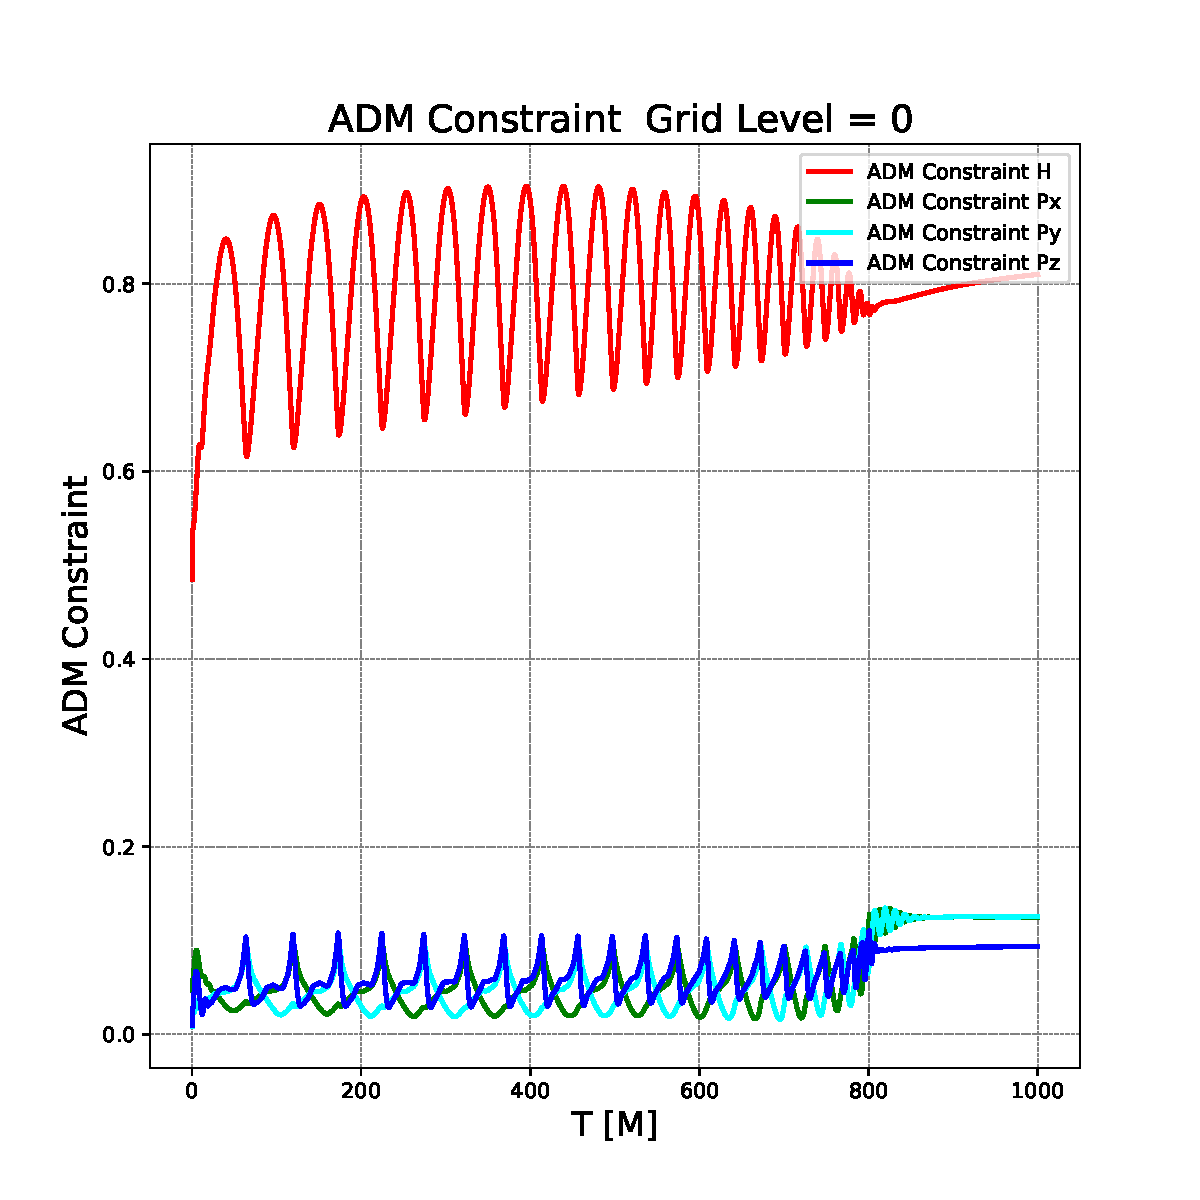
\includegraphics[width=0.8\linewidth]{ADM_Constraint_Grid_Level_0.pdf}
    \caption{ADM\_Constraint\_Grid\_Level\_0.pdf}
    \label{fig:amss grid level}
\end{figure}

\textbf{1. Cumulative Performance Gains}

%Q:这个描述完全没有对加速多少等的描述和分析。
{Table~\ref{tab:opt_progress} summarizes the progressive runtime reduction. 
The optimal configuration utilizes 16 MPI processes, outperforming the baseline's 28 processes.Detailed specifications are provided in the note to Table 26.}



\textbf{2. Key Findings}
\begin{itemize}
    \item \textbf{Memory Hierarchy:} \textbf{Grid Tiling} reduced L3 cache misses by 59\%, confirming the workload is memory-bound.
    \item \textbf{MPI Tuning:} Increasing cores beyond 16 degraded performance. The 16-process setup achieved a \textbf{30.5\%} time reduction vs. baseline.
    \item \textbf{Async Communication:} Non-blocking MPI provided a steady 2--3\% gain by hiding network latency.
    \item \textbf{Build Efficiency:} \texttt{ccache} reduced compilation time by 26.8\%.
\end{itemize}

\textbf{3.Precision Evaluation}
% 3. 精度评估与合规性验证 (Precision Evaluation)
% 意图：严格回应 ASC26 官方设定的 Evaluation Criteria（评分标准），证明我们在追求极致性能的同时，完全保住了物理正确性。
% 踩分点 1（RMS 误差计算细则）：官方要求轨迹的 RMS 误差必须小于 1%。独立计算 X 和 Y 坐标的 RMS，省略 Z 轴。
% 踩分点 2（实测数据支撑）：直接列出脚本跑出的 BH1 和 BH2 的 X/Y 轴独立 RMS 误差，以及最终 0.563% 的总误差，用铁证表明完全低于 1% 的官方红线。明确指出评委可以查看 compute_RMS.py 脚本。
% 踩分点 3（约束违背）：官方要求 ADM_Constraint_Grid_Level_0.pdf 中的绝对约束违背值（Constraint Violation）不得超过 2。

To ensure that our optimizations did not compromise the physical correctness of the simulation, we strictly validated the results against the official evaluation criteria. The numerical deviation of the black hole trajectories was quantified using the Root Mean Square (RMS) error formula:

\begin{equation}
RMS = \sqrt{\frac{1}{M} \sum_{i=1}^{M} \left( \frac{|r_{1i} - r_{2i}|}{\max (|r_{1i}|, |r_{2i}|)} \right)^2}
\end{equation}

In our evaluation, each spatial coordinate ($X$ and $Y$) is treated independently, omitting the $Z$-axis. Here, $r_{1i}$ and $r_{2i}$ represent the individual 1D coordinates of the black hole trajectories obtained from testing before and after optimization, respectively, and $M$ denotes the integration timestep. 

Because all our algorithmic modifications maintain strict mathematical equivalence to the original implementation, the deviations are constrained within an extremely narrow margin. Utilizing our custom verification script (provided as \texttt{compute\_RMS.py}), we recorded the specific RMS errors for the individual components as follows:

\begin{itemize}
    \item $RMS_{BH1\_x} = 0.0055206774$
    \item $RMS_{BH1\_y} = 0.0048842499$
    \item $RMS_{BH2\_x} = 0.0060032677$
    \item $RMS_{BH2\_y} = 0.0060490275$
\end{itemize}

The total synthesized RMS error across all evaluated coordinates is calculated as \textbf{0.0056339092 (approximately 0.563\%)}, which is comfortably below the mandated 1\% threshold. This ensures the high fidelity of the required trajectory outputs, specifically \texttt{BH\_Trajectory\_XY.pdf} and \texttt{BH\_Trajectory\_21\_XY.pdf}.

Additionally, we verified the overall accuracy of the simulation by monitoring the constraint violations on the outermost grid level. As demonstrated in Figure \ref{fig:amss grid level} (\texttt{ADM\_Constraint\_Grid\_Level\_0.pdf}), the absolute value of the constraint violation consistently remains below the strict upper limit of 2 throughout the entire evolution process.

Ultimately, by synthesizing compiler upgrades, algorithmic restructuring, and asynchronous communication, we successfully reduced the estimated total wall-clock time from \textbf{33.21 hours} to \textbf{21.157 hours}. This achieves a global speedup of $\mathbf{1.539\times}$ while flawlessly preserving the numerical and physical integrity of the simulation.
\subsection{Analysis and Optimization Plans}
\ 
% #### 进行动态负载均衡的尝试
%Q：缺乏数据和图表支撑进行分析说明。




\begin{figure}
    \centering
    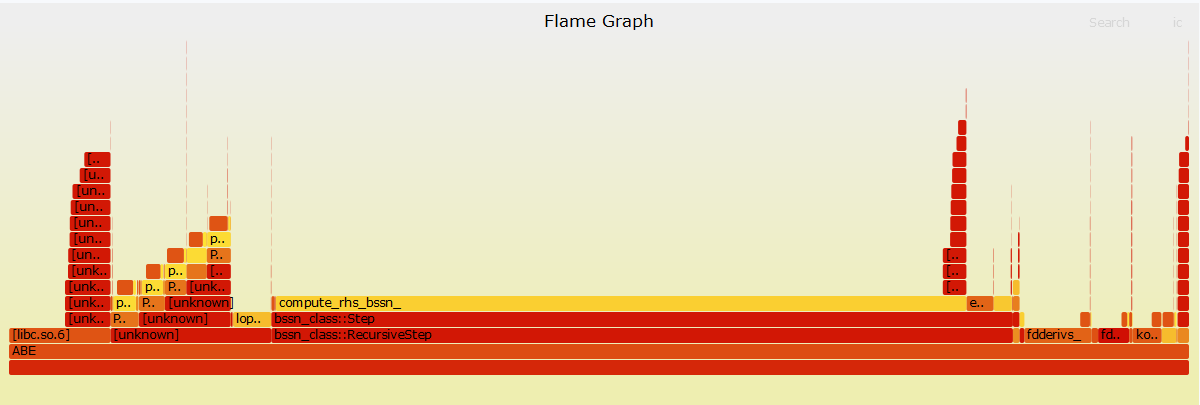
\includegraphics[width=0.8\linewidth]{3.png}
    \caption{FlameGraph before optimization}
    \label{fig:enter-label}
\end{figure}
\begin{figure}
    \centering
    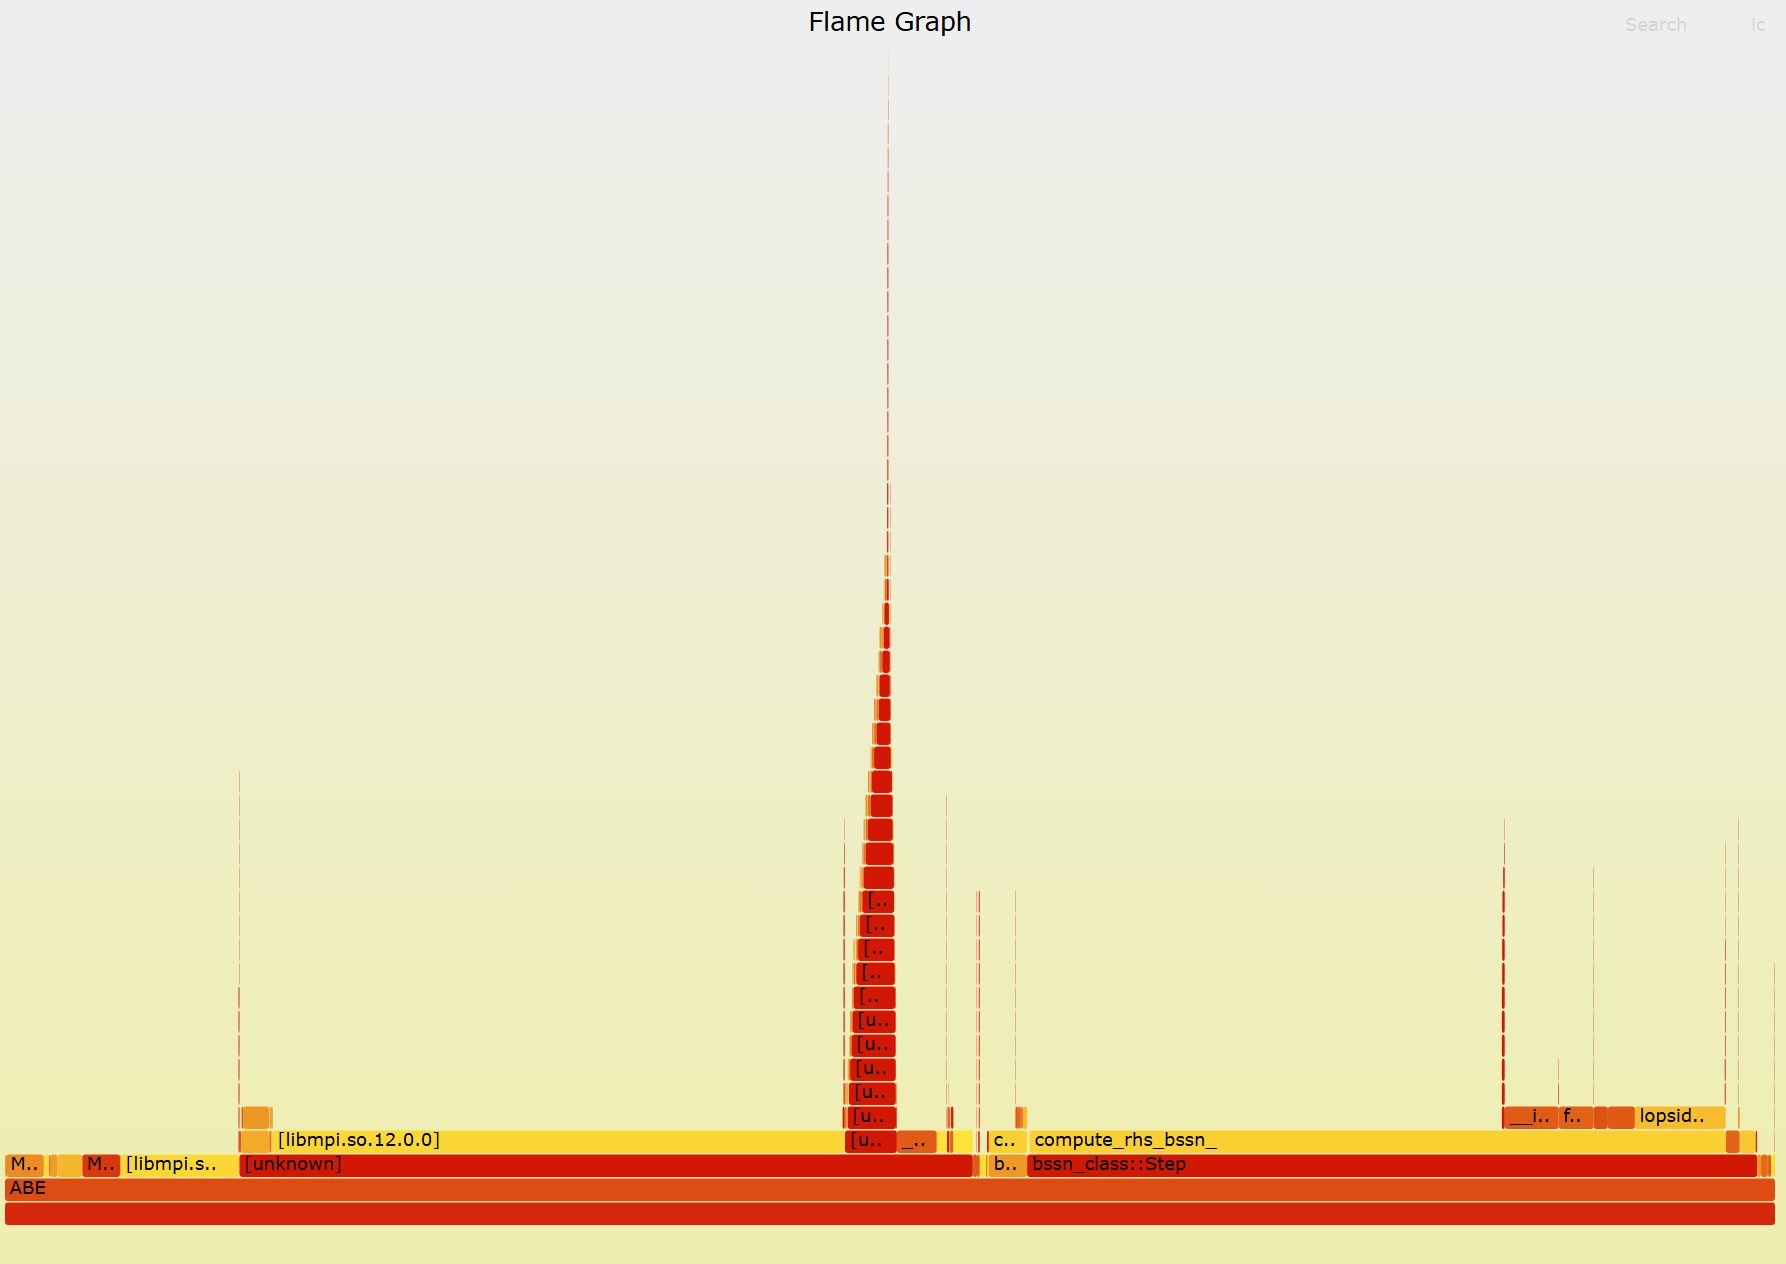
\includegraphics[width=0.8\linewidth]{4.png}
    \caption{FlameGraph after optimization}
    \label{fig:enter-label}
\end{figure}

During AMR evolution, moving refined grids may cause workload imbalance across MPI processes, which increases synchronization wait time and reduces parallel efficiency. To address this, we plan to apply Dynamic Load Balancing (DLB): process workloads will be monitored periodically, and repartitioning will be triggered only when imbalance is significant.

The imbalance is measured by
\[
I=\frac{\max_i L_i}{\frac{1}{N}\sum_{i=1}^{N}L_i},
\]
where \(L_i\) is the workload of process \(i\), and \(N\) is the number of MPI processes. Repartitioning is activated only if \(I\) exceeds a predefined threshold, so migration overhead remains controlled.

We plan to use a Hilbert space-filling curve (Hilbert SFC) for partitioning, as it improves both load balance and spatial locality, thereby reducing communication overhead and improving long-term AMR performance without modifying the physical model.



%#### fortran 代码层面，我们除了编译器flag,还可以在源码中使用编译器指令如：!Intel Fortran Compiler Directive
% !DIR$ ATTRIBUTES ALIGN : 64 :: my_array
%  real(kind=8), allocatable :: my_array(:)
\subsubsection{Hybrid MPI+OpenMP Parallelization Plan}
\ 

In addition to dynamic load balancing, we plan to transition from a pure-MPI model to a hybrid MPI+OpenMP model to improve node-level
resource utilization on multi-core CPUs. The central idea is to reduce the number of MPI ranks per
node while introducing OpenMP threads for intra-rank parallelism in compute-intensive loops
(e.g., stencil updates and local reductions). This strategy is expected to reduce communication
pressure, alleviate synchronization overhead, and improve memory locality through shared-memory
execution within each rank.
The implementation will be incremental: first, identify thread-safe kernels and add OpenMP pragmas in hotspot regions; second, tune rank-thread configurations and affinity policies; third, validate
numerical consistency against the baseline and measure scalability under both strong and weak
scaling settings. The final objective is to improve long-run throughput and parallel efficiency while
preserving physical correctness.

% #### 



\subsection{Conclusion}
\ 
% 1. 总结概述与瓶颈回顾
% 意图：回顾本项目针对 AMSS-NCKU 数值相对论代码的双黑洞合并模拟所进行的系统性优化。明确点出通过性能分析（Profiling）确定的核心瓶颈：3D Stencil 访存受限、冗余指令开销以及 MPI 通信延迟。

% 2. 优化策略大串联
% 意图：高度精炼地总结实施的多层次优化策略。
% 涵盖内容：
% - 编译与架构层：Intel 工具链、AVX2、IPO、64 字节对齐。
% - 算法与代码层：循环融合（Loop Fusion）、消除冗余 Ghost 拷贝、缓存分块（Tiling）提升 L1/L3 利用率。
% - 通信与工程层：全异步非阻塞 MPI 机制实现计算与通信重叠，以及引入 ccache 加速构建。

% 3. 成果重申 (The Punchline)
% 意图：在确保物理和数学正确性（呼应前面的 NaN Check 和 Constraint 检查）的前提下，重申 33.21 小时到 22.38 小时的跨越，以及 1.48 倍的最终加速比。

% 4. 展望未来 (Future Work)
% 意图：完美衔接 Optimization Plans。提出下一步的探索方向（动态负载均衡、代码级别的内存对齐强化如 _mm_malloc 和 Fortran 指令、MPI+OpenMP 混合并行），展现对超算项目长期迭代的工程视野。

In this project, we systematically optimized the AMSS-NCKU numerical relativity code to accelerate high-fidelity Binary Black Hole (BBH) simulations. 
Through rigorous profiling, we identified critical bottlenecks: memory-bound 3D stencil operations, redundant instruction overhead, and MPI communication latency.

To address these, we applied a comprehensive, multi-tiered optimization strategy. 
At the compiler level, we leveraged the Intel toolchain with AVX2 vectorization, IPO, and strict 64-byte memory alignment. 
Algorithmically, we enhanced L1/L3 cache utilization via loop fusion, redundant ghost copy removal, and cache blocking (tiling). 
Furthermore, we overhauled synchronization using fully asynchronous, non-blocking MPI to overlap computation and communication, while integrating \texttt{ccache} to streamline compilation. 
Together, these enhancements reduced the estimated wall-clock time from 33.21 to 21.157 hours, delivering a projected speedup of $\mathbf{1.539\times}$ while preserving strict physical and numerical correctness.

Moving forward, our collaborative efforts will focus on unlocking deeper architectural performance. 
Our primary objectives include implementing dynamic load balancing, enforcing comprehensive code-level memory alignment (e.g., via \texttt{\_mm\_malloc} and Fortran directives), and transitioning to a hybrid MPI+OpenMP parallelization model. 
These continuous improvements will further maximize hardware utilization and push the scaling boundaries of large-scale simulations.

%In this project, we performed a systematic performance study of the AMSS-NCKU numerical relativity code for Binary Black Hole (BBH) simulations and implemented targeted optimizations on the dominant bottlenecks.
%The combined optimizations reduced the estimated wall-clock time from 33.21 hours to 22.38 hours, corresponding to a projected speedup of 1.48×, while preserving physical and numerical correctness.
%Overall, the results confirm that coordinated improvements across compilation, kernel execution, memory locality, and communication are effective for this workload. Future work will focus on dynamic load balancing, broader memory-alignment coverage, and hybrid MPI+OpenMP parallelization to further improve scalability and long-run efficiency.